\documentclass[11pt]{article}
\usepackage[margin=1.1in]{geometry}
\usepackage{amsmath,amssymb,amsthm}
\usepackage{booktabs}
\usepackage{pgfplots}\pgfplotsset{compat=1.18}
\usepackage[hidelinks]{hyperref}
\usepackage{microtype}

\newtheorem{proposition}{Proposition}
\newtheorem{corollary}[proposition]{Corollary}
\newtheorem*{remark}{Remark}
\newcommand{\R}{\mathbb{R}}

% generated by make-figures.js — do not edit
\newcommand{\figEnvelope}{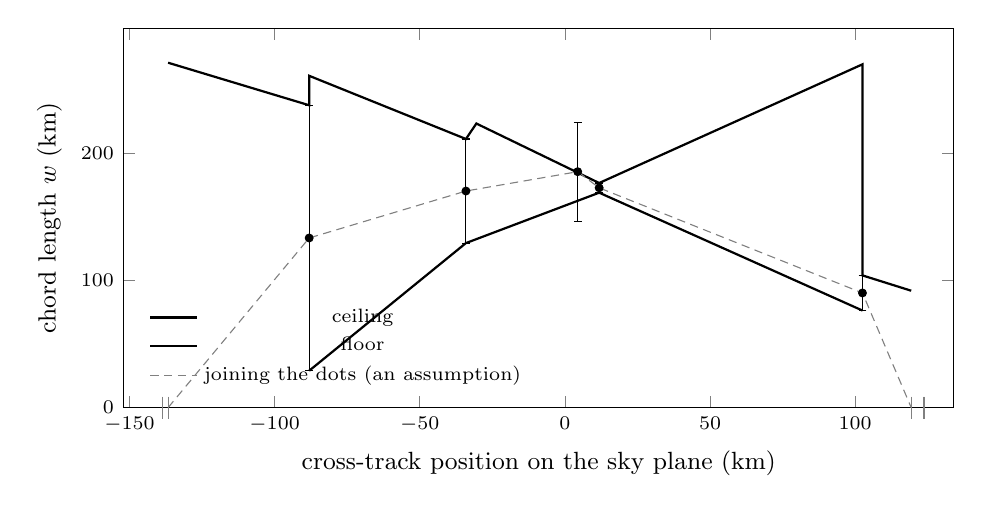
\begin{tikzpicture}
\begin{axis}[width=\linewidth,height=6.4cm,xlabel={cross-track position on the sky plane (km)},
 ylabel={chord length $w$ (km)},xmin=-152,xmax=134,ymin=0,
 tick label style={font=\scriptsize},label style={font=\small},
 legend style={font=\scriptsize,at={(0.02,0.03)},anchor=south west,draw=none,fill=none}]
\addplot[black,thick] coordinates {(-136.7000,271.0216) (-124.7781,262.8231) (-124.7781,262.8231) (-114.3958,255.6833) (-114.3958,255.6833) (-110.4192,252.9486) (-110.4192,252.9486) (-109.4108,252.2552) (-109.4108,252.2552) (-107.7414,251.1071) (-107.7414,251.1071) (-101.8282,247.0407) (-101.8282,247.0407) (-98.8434,244.9881) (-98.8434,244.9881) (-96.6997,243.5139) (-96.6997,243.5139) (-90.3447,239.1436) (-90.3447,239.1436) (-88.1000,237.6000) (-88.1000,260.7471) (-86.4454,259.2259) (-86.4454,259.2259) (-72.1710,246.1021) (-72.1710,246.1021) (-68.9991,243.1859) (-68.9991,243.1859) (-62.0754,236.8203) (-62.0754,236.8203) (-57.0894,232.2362) (-57.0894,232.2362) (-55.5837,230.8519) (-55.5837,230.8519) (-54.8017,230.1329) (-54.8017,230.1329) (-49.3107,225.0846) (-49.3107,225.0846) (-46.8029,222.7789) (-46.8029,222.7789) (-46.7189,222.7017) (-46.7189,222.7017) (-40.2359,216.7412) (-40.2359,216.7412) (-40.0918,216.6088) (-40.0918,216.6088) (-38.6511,215.2842) (-38.6511,215.2842) (-37.4442,214.1746) (-37.4442,214.1746) (-36.7195,213.5084) (-36.7195,213.5084) (-36.3759,213.1924) (-36.3759,213.1924) (-34.1000,211.1000) (-34.1000,211.1000) (-31.5920,219.5574) (-31.5920,219.5574) (-30.5021,223.2329) (-30.5021,223.2329) (-28.1925,220.6813) (-28.1925,220.6813) (-26.2403,218.5247) (-26.2403,218.5247) (-24.4453,216.5417) (-24.4453,216.5417) (-23.3881,215.3737) (-23.3881,215.3737) (-22.4654,214.3544) (-22.4654,214.3544) (-21.7263,213.5379) (-21.7263,213.5379) (-20.7745,212.4863) (-20.7745,212.4863) (-19.4699,211.0451) (-19.4699,211.0451) (-18.1689,209.6079) (-18.1689,209.6079) (-17.6569,209.0423) (-17.6569,209.0423) (-17.5962,208.9752) (-17.5962,208.9752) (-16.1645,207.3935) (-16.1645,207.3935) (-15.2238,206.3543) (-15.2238,206.3543) (-14.3922,205.4356) (-14.3922,205.4356) (-13.6032,204.5639) (-13.6032,204.5639) (-13.3431,204.2767) (-13.3431,204.2767) (-12.1500,202.9585) (-12.1500,202.9585) (-11.6618,202.4192) (-11.6618,202.4192) (-11.5639,202.3111) (-11.5639,202.3111) (-11.3516,202.0765) (-11.3516,202.0765) (-11.1297,201.8314) (-11.1297,201.8314) (-11.0865,201.7837) (-11.0865,201.7837) (-10.9880,201.6749) (-10.9880,201.6749) (-10.4375,201.0667) (-10.4375,201.0667) (-9.9668,200.5467) (-9.9668,200.5467) (-7.9478,198.3162) (-7.9478,198.3162) (-6.7655,197.0101) (-6.7655,197.0101) (-6.7123,196.9513) (-6.7123,196.9513) (-6.3182,196.5159) (-6.3182,196.5159) (-5.6403,195.7670) (-5.6403,195.7670) (-3.9026,193.8473) (-3.9026,193.8473) (-3.3867,193.2773) (-3.3867,193.2773) (-1.6735,191.3847) (-1.6735,191.3847) (-1.3033,190.9757) (-1.3033,190.9757) (-1.1299,190.7842) (-1.1299,190.7842) (-0.7055,190.3154) (-0.7055,190.3154) (0.3438,189.1561) (0.3438,189.1561) (1.4529,187.9308) (1.4529,187.9308) (1.7073,187.6498) (1.7073,187.6498) (4.4000,184.6751) (4.4000,184.6751) (6.4926,182.3633) (6.4926,182.3633) (7.0292,181.7705) (7.0292,181.7705) (7.3711,181.3928) (7.3711,181.3928) (7.4446,181.3116) (7.4446,181.3116) (7.4582,181.2966) (7.4582,181.2966) (7.8980,180.8107) (7.8980,180.8107) (8.2883,180.3796) (8.2883,180.3796) (8.3346,180.3283) (8.3346,180.3283) (8.6279,180.0044) (8.6279,180.0044) (9.6840,178.8376) (9.6840,178.8376) (10.2018,178.2656) (10.2018,178.2656) (10.2114,178.2549) (10.2114,178.2549) (10.2760,178.1836) (10.2760,178.1836) (10.6116,177.8129) (10.6116,177.8129) (10.9089,177.4845) (10.9089,177.4845) (10.9533,177.4353) (10.9533,177.4353) (11.1430,177.2258) (11.1430,177.2258) (11.8000,176.5000) (11.8000,176.5000) (12.2752,176.9887) (12.2752,176.9887) (14.1811,178.9485) (14.1811,178.9485) (15.4376,180.2406) (15.4376,180.2406) (16.3741,181.2037) (16.3741,181.2037) (17.8033,182.6733) (17.8033,182.6733) (18.3811,183.2675) (18.3811,183.2675) (18.3854,183.2719) (18.3854,183.2719) (20.6313,185.5814) (20.6313,185.5814) (24.0995,189.1479) (24.0995,189.1479) (24.5509,189.6120) (24.5509,189.6120) (26.2713,191.3812) (26.2713,191.3812) (30.0231,195.2392) (30.0231,195.2392) (30.3709,195.5969) (30.3709,195.5969) (31.3830,196.6376) (31.3830,196.6376) (34.3200,199.6578) (34.3200,199.6578) (34.7235,200.0728) (34.7235,200.0728) (35.6790,201.0553) (35.6790,201.0553) (35.7615,201.1401) (35.7615,201.1401) (43.4889,209.0864) (43.4889,209.0864) (44.2949,209.9153) (44.2949,209.9153) (52.6437,218.5005) (52.6437,218.5005) (52.8033,218.6646) (52.8033,218.6646) (53.2282,219.1015) (53.2282,219.1015) (60.7028,226.7878) (60.7028,226.7878) (61.3986,227.5033) (61.3986,227.5033) (63.1783,229.3335) (63.1783,229.3335) (64.6756,230.8731) (64.6756,230.8731) (65.7277,231.9550) (65.7277,231.9550) (67.6970,233.9802) (67.6970,233.9802) (68.0378,234.3306) (68.0378,234.3306) (72.4607,238.8788) (72.4607,238.8788) (76.8602,243.4029) (76.8602,243.4029) (77.4284,243.9871) (77.4284,243.9871) (80.2284,246.8664) (80.2284,246.8664) (81.6500,248.3283) (81.6500,248.3283) (82.4970,249.1993) (82.4970,249.1993) (84.0719,250.8188) (84.0719,250.8188) (86.8954,253.7222) (86.8954,253.7222) (87.9939,254.8519) (87.9939,254.8519) (88.4881,255.3601) (88.4881,255.3601) (91.5159,258.4737) (91.5159,258.4737) (102.5000,269.7688) (102.5000,103.9000) (104.9307,102.1581) (104.9307,102.1581) (107.7352,100.1482) (107.7352,100.1482) (112.8229,96.5021) (112.8229,96.5021) (119.3000,91.8603)};
\addlegendentry{ceiling}
\addplot[black,thick] coordinates {(-88.1000,29.0000) (-34.1000,129.3000) (11.8000,168.9000) (102.5000,76.3000)};
\addlegendentry{floor}
\addplot[gray,densely dashed] coordinates {(-136.7000,0.0000) (-88.1000,133.3000) (-34.1000,170.2000) (4.4000,185.4000) (11.8000,172.7000) (102.5000,90.1000) (119.3000,0.0000)};
\addlegendentry{joining the dots (an assumption)}
\addplot[only marks,mark=*,mark size=1.4pt,black,error bars/.cd,y dir=both,y explicit]
  coordinates {(102.50,90.10) +- (0,13.80)};
\addplot[only marks,mark=*,mark size=1.4pt,black,error bars/.cd,y dir=both,y explicit]
  coordinates {(11.80,172.70) +- (0,3.80)};
\addplot[only marks,mark=*,mark size=1.4pt,black,error bars/.cd,y dir=both,y explicit]
  coordinates {(4.40,185.40) +- (0,39.00)};
\addplot[only marks,mark=*,mark size=1.4pt,black,error bars/.cd,y dir=both,y explicit]
  coordinates {(-34.10,170.20) +- (0,40.90)};
\addplot[only marks,mark=*,mark size=1.4pt,black,error bars/.cd,y dir=both,y explicit]
  coordinates {(-88.10,133.30) +- (0,104.30)};
\addplot[only marks,mark=|,mark size=4pt,gray] coordinates {(123.90,0)};
\addplot[only marks,mark=|,mark size=4pt,gray] coordinates {(123.60,0)};
\addplot[only marks,mark=|,mark size=4pt,gray] coordinates {(119.30,0)};
\addplot[only marks,mark=|,mark size=4pt,gray] coordinates {(-136.70,0)};
\addplot[only marks,mark=|,mark size=4pt,gray] coordinates {(-138.70,0)};
\addplot[only marks,mark=|,mark size=4pt,gray] coordinates {(-182.00,0)};
\addplot[only marks,mark=|,mark size=4pt,gray] coordinates {(-188.80,0)};
\end{axis}
\end{tikzpicture}}
\newcommand{\figLadder}{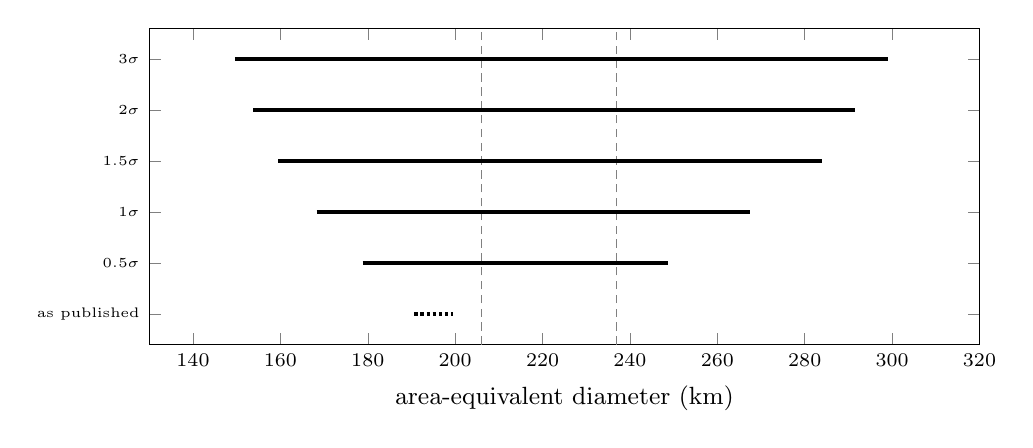
\begin{tikzpicture}
\begin{axis}[width=\linewidth,height=5.6cm,xlabel={area-equivalent diameter (km)},
 ytick={1,2,3,4,5,6},
 yticklabels={as published,$0.5\sigma$,$1\sigma$,$1.5\sigma$,$2\sigma$,$3\sigma$},
 ymin=0.4,ymax=6.6,xmin=130,xmax=320,
 tick label style={font=\scriptsize},label style={font=\small},y tick label style={font=\tiny}]
\addplot[draw=none] coordinates {(130,1)};
\draw[gray,densely dashed] (axis cs:206,0.4) -- (axis cs:206,6.6);
\draw[gray,densely dashed] (axis cs:237,0.4) -- (axis cs:237,6.6);
\draw[very thick,densely dotted] (axis cs:190.67,1) -- (axis cs:199.46,1);
\draw[very thick] (axis cs:178.80,2) -- (axis cs:248.79,2);
\draw[very thick] (axis cs:168.27,3) -- (axis cs:267.54,3);
\draw[very thick] (axis cs:159.54,4) -- (axis cs:283.95,4);
\draw[very thick] (axis cs:153.76,5) -- (axis cs:291.58,5);
\draw[very thick] (axis cs:149.61,6) -- (axis cs:299.05,6);
\end{axis}
\end{tikzpicture}}


\title{What a stellar occultation forces about a body's size\\
when only its silhouette's convexity is assumed}
\author{Carlos Toledo\thanks{Contact: carlos@carlostoledo.co.
Preprint v1.0. % [OWNER: affiliation, acknowledgments and any AI-assistance
% disclosure wording are yours to set before deposit.]
}}
\date{September 2026}

\begin{document}
\maketitle

\begin{abstract}
A stellar occultation gives a handful of parallel chords across a small body's
silhouette, and the size that gets published is an ellipse fitted to them. We
ask what the chords force on their own. Because occultation chords are parallel
and a convex silhouette has a concave upper boundary and a convex lower one, the
chord length $w(y)$ is a \emph{concave} function of the cross-track coordinate,
vanishing outside the body's support; the silhouette's area is $\int w$. The
problem is therefore one-dimensional and closed form, with no optimiser and no
convergence, and on published decimal data every bound is an exact rational.
Applied to the 2017 May 20 occultation by the centaur (95626)~2002~GZ$_{32}$,
convexity alone forces the area-equivalent diameter into
$[168.3,\,267.5]$\,km, against a published $206\pm15$\,km. Two facts fall out.
At face value the five chords admit \emph{no} convex silhouette at all --- the
concave hull of the measured lengths runs $5.5$\,km above one station's own
chord --- and about half of one stated error bar is needed before one exists.
And the bound is asymmetric by construction: the floor is bought by the chords,
while the ceiling is bought entirely by the telescopes that recorded
\emph{nothing}. Moving this campaign's 23 negative stations out of reach raises
the ceiling from $267.5$ to $577.0$\,km.
\end{abstract}

\section{The chord-length function}

Occultation chords are parallel: the shadow sweeps in one direction and every
station cuts the silhouette along that direction. Take that direction as $x$ and
let $y$ be the cross-track coordinate. Let $K\subset\R^2$ be the silhouette,
assumed compact and convex, with slices
$K\cap\{y\}=[L(y),R(y)]$ on its support $[Y^-,Y^+]$.

\begin{proposition}\label{prop:concave}
$R$ is concave and $L$ is convex on $[Y^-,Y^+]$, so the chord length
$w=R-L$ is concave there and zero outside; and $\operatorname{area}(K)=\int w$.
\end{proposition}

\begin{proof}
For $y_1,y_2$ in the support and $t\in[0,1]$, the points $(R(y_1),y_1)$ and
$(R(y_2),y_2)$ lie in $K$, so their combination does too, giving
$R(ty_1+(1-t)y_2)\ge tR(y_1)+(1-t)R(y_2)$; the same argument with $L$ reverses
the inequality. The area statement is Fubini.
\end{proof}

\begin{remark}
Convexity is weaker than the ellipse that occultation papers fit, and it is
already asserted by the data: a single ingress and a single egress per station
is what a convex silhouette produces. It is also capable of being wrong, which
is what makes it an assumption worth naming --- a dumbbell has a chord-length
function that is not concave, and the construction below excludes it.
\end{remark}

Write the measurements as $w(y_i)\in[\ell_i-\varepsilon_i,\,\ell_i+\varepsilon_i]$
at $n$ cross-track positions, and let $y^-<\min_i y_i$ and $y^+>\max_i y_i$ be
the nearest stations that observed and saw nothing, so that
$[Y^-,Y^+]\subseteq[y^-,y^+]$.

\section{The two bounds, and why they are asymmetric}

\begin{proposition}[floor]\label{prop:floor}
Let $\widehat{w}$ be the concave hull of the points $(y_i,\ell_i-\varepsilon_i)$
on $[y_1,y_n]$. Then $\operatorname{area}(K)\ge\int_{y_1}^{y_n}\widehat{w}$, and
the bound is attained.
\end{proposition}

\begin{proof}
$w$ is concave on a support containing $[y_1,y_n]$ and satisfies
$w(y_i)\ge\ell_i-\varepsilon_i$, so it dominates the smallest concave function
through those points; and $w\ge0$ elsewhere. Attainment: the convex hull of the
chords themselves is a convex body realising it.
\end{proof}

\begin{remark}
The negative stations do not appear. Nothing forces the body past its outermost
chord: it may end flush with it, giving a flat edge, which is a perfectly good
convex body. In particular the polygon obtained by ``joining the dots'' down to
the negative stations is \emph{not} a lower bound --- it already assumes the
body reaches them.
\end{remark}

\begin{proposition}[ceiling]\label{prop:ceiling}
For $y\notin[y_i,y_j]$ with $y_i<y_j$,
\begin{equation}
w(y)\;\le\;U_{ij}(y)\;:=\;
\begin{cases}
(\ell_j+\varepsilon_j)+\dfrac{(\ell_j+\varepsilon_j)-(\ell_i-\varepsilon_i)}{y_j-y_i}(y-y_j), & y>y_j,\\[2ex]
(\ell_i+\varepsilon_i)+\dfrac{(\ell_i+\varepsilon_i)-(\ell_j-\varepsilon_j)}{y_i-y_j}(y-y_i), & y<y_i,
\end{cases}
\end{equation}
and consequently
$\operatorname{area}(K)\le\int_{y^-}^{y^+}\max\!\big(0,\min_{ij}U_{ij}\big)$.
\end{proposition}

\begin{proof}
For $y_i<y_j<y$, concavity of $w$ on the support gives
$w(y_j)\ge\frac{(y-y_j)w(y_i)+(y_j-y_i)w(y)}{y-y_i}$; solving for $w(y)$ gives a
bound in which $w(y_j)$ carries a positive coefficient and $w(y_i)$ a negative
one, so the largest admissible value uses $\ell_j+\varepsilon_j$ and
$\ell_i-\varepsilon_i$. The other case is symmetric. Outside $[y^-,y^+]$ the
body is absent, so $w=0$ there.
\end{proof}

\begin{remark}[the negatives are not samples]
It is tempting to enter $y^\pm$ into the pair list as ordinary samples with
$w=0$. That is unsound. $w$ is concave \emph{on its support} and zero outside;
a function that is zero on two rays and concave between them is not concave. On
a triangular silhouette, admitting the far cap as a sample produced a ceiling of
$7529$ against a true area of $9000$, because the cap dragged the envelope down
through the body itself. The negative stations clip the domain of integration
and nothing else --- and that is already the whole of what they buy.
\end{remark}

\begin{remark}[the ceiling is discontinuous]
The constraints anchored at a sample are valid only up to it, so
$\min_{ij}U_{ij}$ jumps upward the instant $y$ passes a chord. Integrating it as
a polyline through the sample points understates the area --- by $16\%$ on a
circle --- and makes the ceiling \emph{fall} when chords are removed, which is
the wrong direction and is how the error was found. Between breakpoints the
envelope is affine, so the midpoint rule is exact and blind to the jumps.
\end{remark}

\section{(95626) 2002 GZ$_{32}$, 2017 May 20}

The campaign of Santos-Sanz et al.\ (2021) is used because its site table
publishes, for every station, the projected distance on the sky plane to the
reconstructed centerline in kilometres together with the detection status. That
column is the cross-track coordinate, already reduced, so no ephemeris, station
projection or Earth-rotation model enters here. Five chords were positive and 23
stations saw nothing. A timing shift slides a chord along its own line and does
not change its length, so nothing below depends on which of the paper's two fits
--- ``original'' ($\chi^2=29.5$) or ``shifted'' ($\chi^2=4.0$) --- one prefers.

\begin{figure}[t]\centering\figEnvelope
\caption{The five chords with their published errors, the 23 stations that saw
nothing (ticks at zero), and the certified envelopes. Joining the dots is drawn
dashed because it is an assumption, not a bound.}\end{figure}

\begin{figure}[t]\centering\figLadder
\caption{Certified area-equivalent diameter against the error budget. The top
bar is dotted because at face value no convex silhouette fits the chords.
Vertical lines: the published ellipse $206$\,km and the radiometric
$237$\,km.}\end{figure}

At the published $1\sigma$ chord errors, convexity alone gives
\[
D_{\mathrm{eq}}\in[168.3,\,267.5]\ \mathrm{km},
\]
against a published $206\pm15$\,km. Two consequences are worth stating.

\emph{The chords are not consistent with convexity as published.} At zero error
the concave hull of the measured lengths runs $5.5$\,km above the Javalambre
chord; about half of one stated error bar admits a convex body. The published
analysis meets the same fact from the other side and records it as
$\chi^2=29.5$.

\emph{A disagreement in the literature dissolves.} The paper reports its
occultation diameter and notes that its mean three-dimensional estimate is not in
agreement with the radiometric $237\pm8$\,km from Herschel, Spitzer and ALMA.
Both values lie inside the certified interval. The tension is between two
models, not between two measurements.

\emph{What the misses are worth.} Moving the 23 negative stations out of reach
raises the ceiling from $267.5$ to $577.0$\,km. The telescopes that recorded
nothing are worth $309$\,km of upper bound --- more than the body's own diameter
--- and they are the part of a campaign least often published.

\section{Limitations}

Only one event is analysed, because a second requires a campaign that publishes
its cross-track distances; converting a timings-only campaign means redoing the
station projection and Earth rotation, which has a built-in check (the computed
chord lengths must reproduce the published ones) but is a real piece of geometry
with a real chance of a silent error. The position of each chord along its own
line is not used --- it is not published here, and the area bound does not need
it --- but it would tighten the ceiling, because it constrains $L$ and $R$
separately rather than only their difference. A central-symmetry rung, which
would make $w$ symmetric about the centre, is a genuine further constraint and a
genuine test; these bodies are not symmetric, and a refutation would be the
informative outcome.

\end{document}
